\section{Resultados}\label{sec:resultados}

En el siguiente apartado, se muestra la realización de la modulación PAM (tanto muestreo natural como instantáneo) a una señal senoidal, además de esto se muestra como se comporta tal modulación a una transformada de Fourier.


\subsection{Actividad 1}
La siguiente figura es de la señal sinusoidal coseno que nos representa una señal analógica.

\begin{equation} \label{eq:frecuencia_del_coseno_y_muestreo}
\begin{split} 
&Frecuencia\ del\ coseno = 1.000 Hz \\
&frecuencia\ de\ muestreo = 100.000 Hz \\
\end{split} 
\end{equation} 

Para que el coseno durara 2 periodos, se utilizaron las siguientes muestras y así se determino el tiempo de la señal.
\begin{equation} \label{eq:L_Muestras}
\begin{split} 
&L(Muestras) = 200 \\
&t=(0:L-1)/frecuenciaMuestreo \\
\end{split} 
\end{equation} 




\begin{figure}[H]
    \centering
    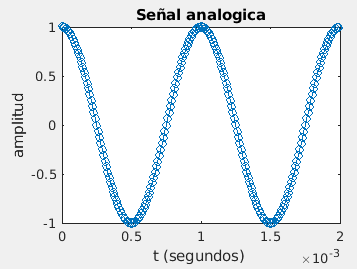
\includegraphics[height=130px, width=180px]{Imagenes/Actividad1/SA.png}
    \caption{Señal analógica}
    \label{fig:Señal_Analógica}
\end{figure}

La siguiente señal es la señal analógica anterior, modulada por muestro Natural, que resulta de (eq:\ref{eq:PAM_muestreo_natural}), donde se utilizaron los siguientes parámetros.

\begin{equation} \label{eq:frecuencia_de_señal_cajo_y_ciclo_de_trabajo}
\begin{split} 
&frecuencia\ de\ señal\ cajón = 5.000 Hz \\
&Ciclo\ de\ trabajo = 70\% \\
\end{split} 
\end{equation} 

\begin{figure}[H]
    \centering
    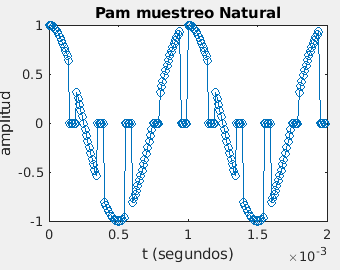
\includegraphics[height=130px, width=180px]{Imagenes/Actividad1/PAMnatural.png}
    \caption{PAM por muestreo natural}
    \label{fig:PAM_por_muestreo_natural}
\end{figure}

La siguiente señal es la señal analógica anterior, modulada por muestro instantáneo, como se puede revisar en (Lineas 20-30) (Anexo código :\ref{ref:codigo1}).

\begin{figure}[H]
    \centering
    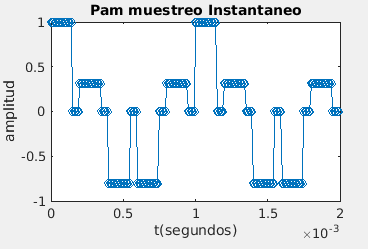
\includegraphics[height=130px, width=180px]{Imagenes/Actividad1/PAMplana.png}
    \caption{PAM por muestreo instantáneo}
    \label{fig:PAM_por_muestreo_instantaneo}
\end{figure}

La siguiente señal es la analógica anterior, pero analizada en el plano de la frecuencia, gracias a la transformada de Fourier. (eq:\ref{eq:Transformada_de_fourier})

\begin{figure}[H]
    \centering
    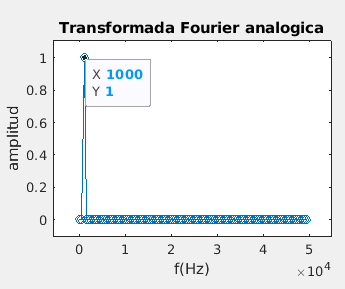
\includegraphics[height=130px, width=180px]{Imagenes/Actividad1/tf.png}
    \caption{Fourier de la señal}
    \label{fig:Fourier_de_la_senal}
\end{figure}

La siguiente señal es la analógica muestreada en PAM natural, pero analizada en el plano de la frecuencia, gracias a la transformada de Fourier. (Ecuación:\ref{eq:Transformada_de_fourier})

\begin{figure}[H]
    \centering
        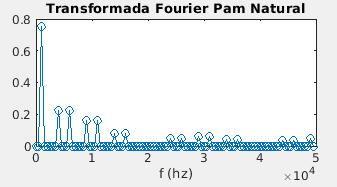
\includegraphics[height=130px, width=180px]{Imagenes/Actividad1/TFnatu.png}
    \caption{Fourier por muestreo natural}
    \label{fig:Fourier_por_muestre_natural}
\end{figure}

La siguiente señal es la analógica muestreada en PAM plana, pero analizada en el plano de la frecuencia, gracias a la transformada de Fourier. (Ecuación:\ref{eq:Transformada_de_fourier})
\begin{figure}[H]
    \centering
    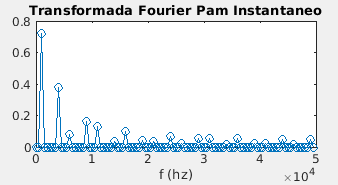
\includegraphics[height=130px, width=180px]{Imagenes/Actividad1/TFplana.png}
    \caption{Fourier por muestreo instantáneo}
    \label{fig:Fourier_por_muestre_natural}
\end{figure}



\subsection{Actividad 2}

En el siguiente apartado se muestra la modulación PCM a la señal trabajada con modulación PAM, además se muestra el resultado gráfico del error de cuantificación de la señal codificada.\\

Los parámetros utilizados para cada procedimiento fueron los siguientes.

\begin{equation} \label{eq:muestras_frecuencia_sinusoidal_muestreo_muestreado}
\begin{split} 
&L(Muestras) = 300 \\
&frecuencia\ sinusoidal=1000; \%Frecuencia\ de\ la\ sinusoidal \\
&frecuencia\ de\ muestreo=100000; \%Frecuencia\ de\ muestreo \\
&\ 1/1e5Hz \\
&tiempo muestreado=0:1/fm:2/fc;
\end{split} 
\end{equation}

\begin{figure}[H]
    \centering
    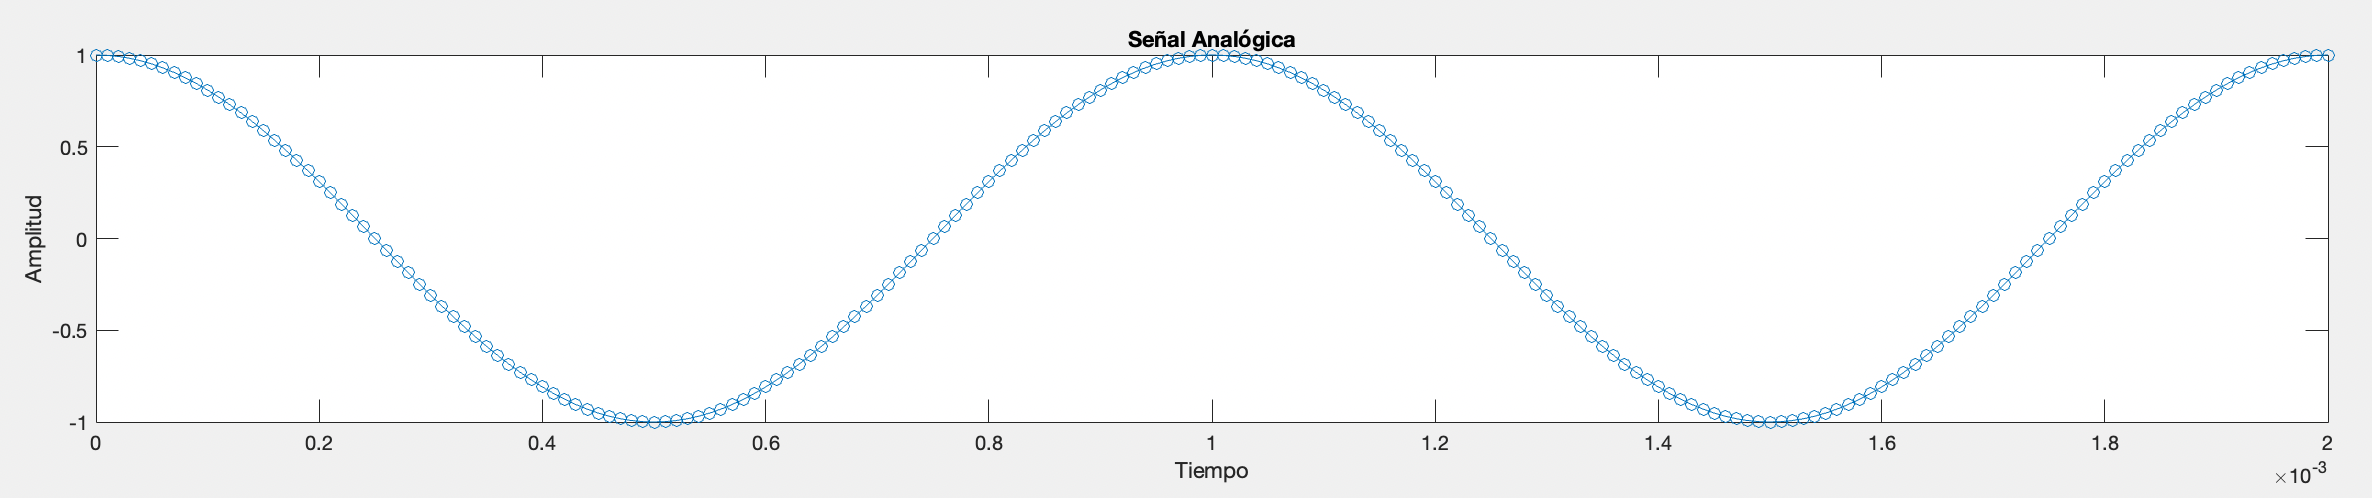
\includegraphics[scale=0.2]{Imagenes/senalanalogica.png}
    \caption{Procedimiento PCM parte 1}
    \label{fig:Procedimiento_PCM_parte_1}
\end{figure}


\begin{figure}[H]
    \centering
    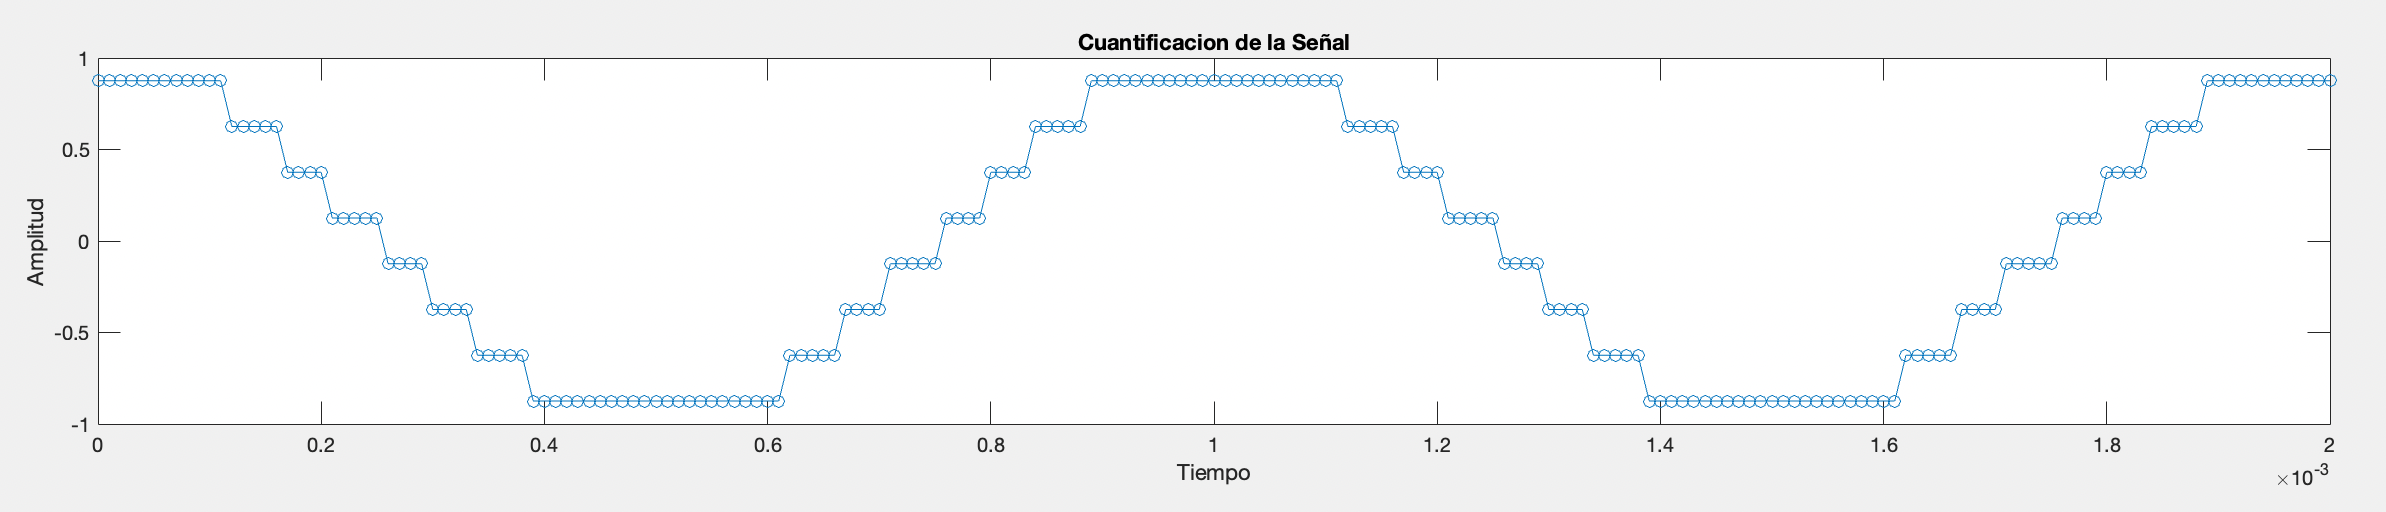
\includegraphics[scale=0.2]{Imagenes/cuantizacion.png}
    \caption{Procedimiento PCM parte 2}
    \label{fig:Procedimiento_PCM_parte_2}
\end{figure}

\begin{figure}[H]
    \centering
    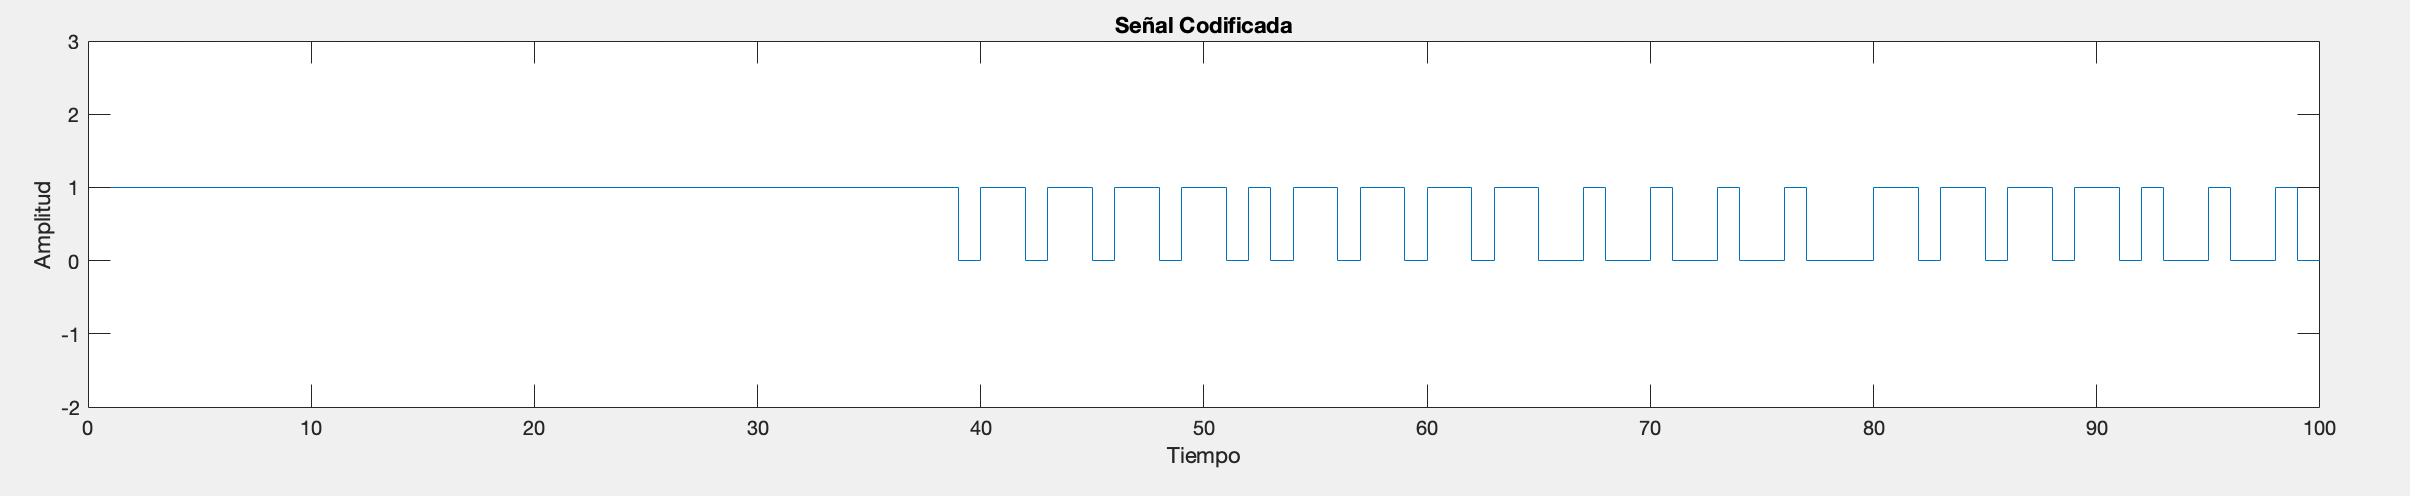
\includegraphics[scale=0.2]{Imagenes/codificacion.png}
    \caption{Procedimiento PCM parte 3}
    \label{fig:Procedimiento_PCM_parte_3}
\end{figure}



Para el apartado siguiente, se utiliza el  parámetro numero de bits  que, directamente afecta el nivel de cuantificación que a su vez mientras mas alto sea el valor del bit menor error de cuantificación habrá.

\begin{equation} \label{eq:frecuencia_de_señal_cajo_y_ciclo_de_trabajo}
\begin{split} 
&numBits=3 \\
&Afectando\ al\ nivel\ de\ cuantificación\ establecido\ por \\ 
&M = 2^{numBits}; \\
\end{split} 
\end{equation}


\begin{figure}[H]
    \centering
    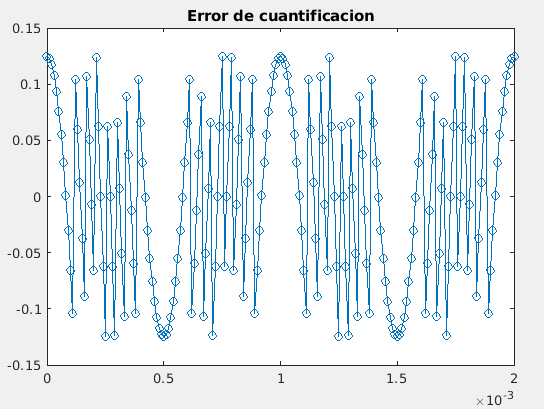
\includegraphics[height=130px, width=180px]{Imagenes/error.png}
    \caption{Error de cuantización con 3 bits}
    \label{fig:Error_de_cuantizacion_con_3_bits}
\end{figure}


\subsection{Cuestionario}

\noindent 

\begin{enumerate}
    \item \textbf{¿Qué pasa si disminuye la frecuencia de muestreo?}\\
    \textbf{R:}
    La señal empieza a perder "suavidad", se asemeja a una señal triangular, resultando en otra señal a la muestra da.
    
    \begin{figure}[H]
        \centering
        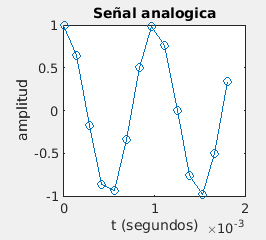
\includegraphics[height=130px, width=180px]{Imagenes/Actividad1/Preguntas/fMinSA.png}
        \caption{Señal analógica con frecuencia de muestro menor}
        \label{fig:fmMinSA}
    \end{figure}
    
    
    \item \textbf{¿Hay algún límite? Si lo hay,¿Cuál es?}\\
    \textbf{R:}
    El limite presente se debe a que la  frecuencia de muestreo debe ser el doble del componente de interés de la frecuencia más alta en la señal estudiada, tal limite de frecuencia se denomina frecuencia de Nyquist, del Teorema de muestreo de Nyquist.\\
    
    \item \textbf{¿Por qué existe ese límite?}\\
    \textbf{R:}
    Al disminuir la frecuencia de muestreo por debajo del la frecuencia Nyquist, la señal estudiada empieza a adoptar una forma de señal triangular, resultando en otra señal.\\
    
    \item \textbf{¿Qué pasa si se supera ese límite?}\\
    \textbf{R:}
    Comienza a aparecer el efecto denominado "Aliasing", que produce que aparezcan frecuencias falsas bajas en los datos muestreados provocando que la señal graficada sea distinta a .\\
    \begin{figure}[H]
        \centering
        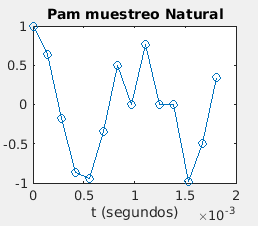
\includegraphics[height=130px, width=180px]{Imagenes/Actividad1/Preguntas/ALIpam.png}
        \caption{Pam natural con Aliasing}
        \label{fig:PlanaAliasing}
    \end{figure}

    \textbf{¿Por qué la transformada de Fourier tiene esa forma?}\\
    \textbf{R:} Al modular la señal produce una disminución del ancho de banda de esta, esto provoca que la señal sea más fácil de transportar.\\
    
    \noindent 
    \textbf{¿El error por cuantificación depende de N  de bits de la palabra PCM?}\\
    \textbf{R:}Si depende, debido a que el error de cuantificación es la diferencia entre el valor real de la muestra (valor analógico) y el nivel asignado, mientras menos bits posea la señal menor serán los niveles asignados por ende el error que se presentará será mayor.
    
\end{enumerate}




